\documentclass[a4paper,11pt]{article}
\usepackage{amsmath}
\usepackage{catoptions}
\usepackage{hyperref}
\usepackage{graphicx}
\usepackage{listings}
\usepackage{color}

\definecolor{gray}{rgb}{0.5,0.5,0.5}
\newcommand{\convolution}{\ensuremath{+\negmedspace\negmedspace\negmedspace\times}}
\newcommand{\highlightColor}{red}

\makeatletter
%% Provide \Autoref; the \autoref with a printed capital
\def\figureautorefname{figure}
\def\tableautorefname{table}
\def\partautorefname{part}
\def\appendixautorefname{appendix}
\def\equationautorefname{equation}
\def\AMSautorefname{equation}
\def\theoremautorefname{theorem}
\def\enumerationautorefname{case}
\def\Autoref#1{%
  \begingroup
  \edef\reserved@a{\cpttrimspaces{#1}}%
  \ifcsndefTF{r@#1}{%
    \xaftercsname{\expandafter\testreftype\@fourthoffive}
      {r@\reserved@a}.\\{#1}%
  }{%
    \ref{#1}%
  }%
  \endgroup
}
\def\testreftype#1.#2\\#3{%
  \ifcsndefTF{#1autorefname}{%
    \def\reserved@a##1##2\@nil{%
      \uppercase{\def\ref@name{##1}}%
      \csn@edef{#1autorefname}{\ref@name##2}%
      \autoref{#3}%
    }%
    \reserved@a#1\@nil
  }{%
    \autoref{#3}%
  }%
}


\makeatother

 
\author{Maarten Inja \and Patrick de Kok}
\title{MLPR: Lab 1}

\lstset{
  language=Octave,
  basicstyle=\footnotesize,
  numbers=left,
  numberstyle=\tiny\color{gray},
  stepnumber=5,
  showspaces=false,
  showstringspaces=true
  showtabs=false,
  frame=single,
  title=\lstname,
  breaklines=true,
}
\begin{document}
\maketitle

\section{The Data}
\begin{figure}[t]
  \begin{center}
    \caption{A plot of the dataset.  The red ``$\color{red}+$'''s represent data points from class A.  The blue ``$\color{blue}\times$'''s represent data points from class B.}
    \label{plot1}
    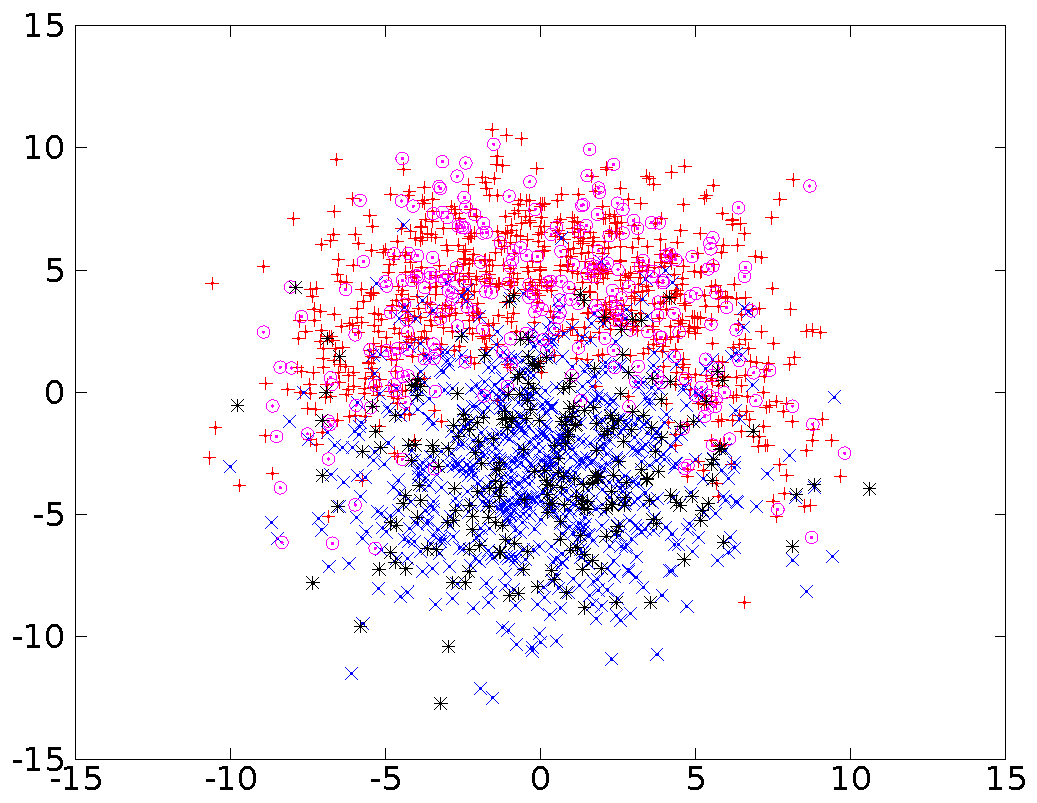
\includegraphics[width=0.6\paperwidth]{plot1}
  \end{center}
\end{figure}

Our training and test data sets are generated through the Matlab code presented in \autoref{code}.  A graphical representation is given in \autoref{plot1}.

\lstinputlisting[caption={The code which generates our data set},label=code]{preprocess_data.m}

\section{$k$NN classifiers}
\label{sec:two}
Our code can be run and experimented with by running the script ``runme'' 
in Matlab\footnote{This script is also supported in Octave} (don't forget to
to set up Netlab!).  
The first two options correspond to this exercise.  

An example to calculate the accuracy for a $k$NN classifier with $k = 1$\footnote{With $k \ge 3$ all accuracies will be returned for $1, 3, \ldots, k$.}
with a test set of 25\%: 
\begin{verbatim}
octave:2> runme
Choose what you want to do

  [ 1] p% split, with data in order
  [ 2] p% split, with data shuffled
  [ 3] n-fold cross-validation, with p% test set and data in order
  [ 4] n-fold cross-validation, with p% test set and data shuffled

pick a number, any number: 2
Which value of k do you want to use? 1
Which percentage of your data do you want to train on? [0-1> 0.75
ans =  0.84200
\end{verbatim}

\begin{enumerate}
\item \textit{Train a $k$NN classifier, with $k$ = 1, on the training data, evaluate its performance on the test data and
compute the test error.}

As can be seen above, the accuracy is \textcolor{\highlightColor}{$0.842$}.  The test error then becomes $1 - 0.842 = \textcolor{\highlightColor}{0.158}$.  

\item \textit{Try other values for $k$ ($k$ = 1, 3, $\ldots$), plot how the test error evolves as a function of $k$ and include the
resulting graph in your report.  Which value of $k$ would you use, and why? Can you derive any definite
conclusions from this experiment?
}

\begin{figure}[t]
  \begin{center}
    \caption{The test error is plotted for odd values of $k$ from 1 to 999.  A closeup for odd values of $k$ from 1 to 19 is given in \autoref{fig:plot3}.}
    \label{fig:plot2}
    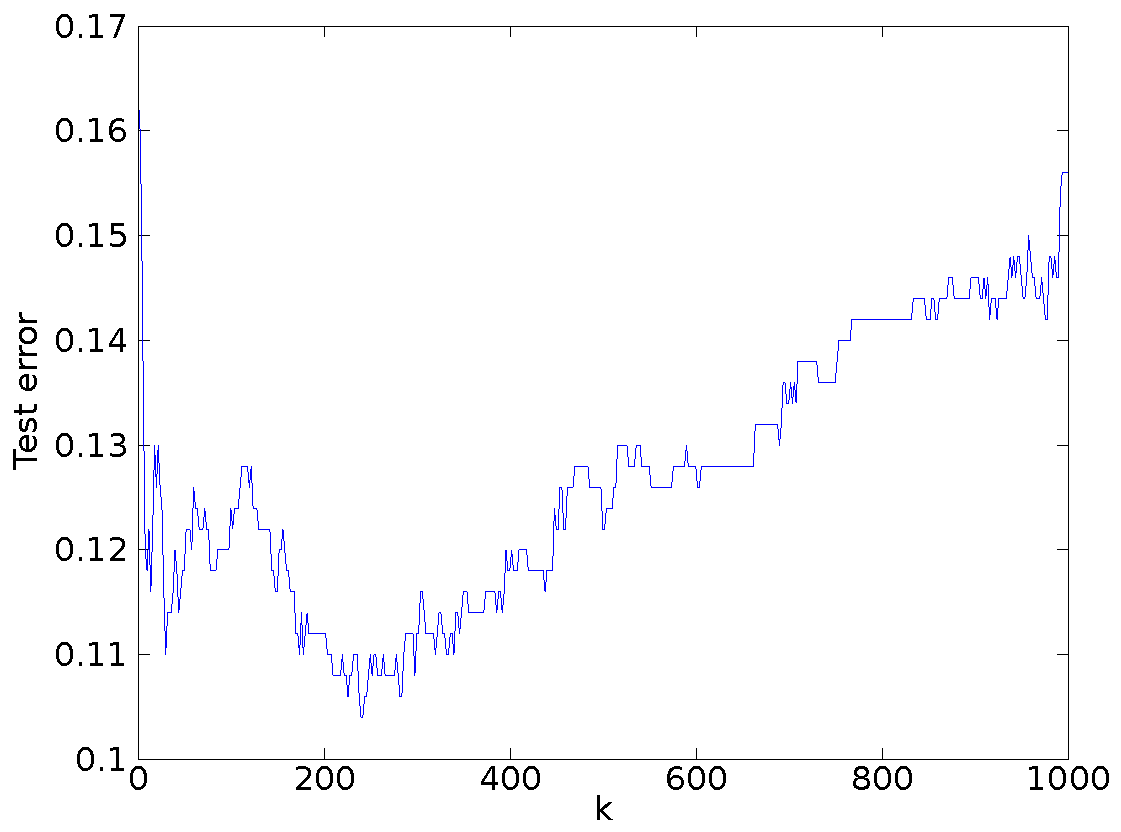
\includegraphics[width=0.6\paperwidth]{plot2.pdf}
  \end{center}
\end{figure}

\begin{figure}[t]
  \begin{center}
    \caption{The test error is plotted for odd values of $k$ from 1 to 19.  A more general overview, for odd values of $k$ from 1 to 999 is given in \autoref{fig:plot2}.}
    \label{fig:plot3}
    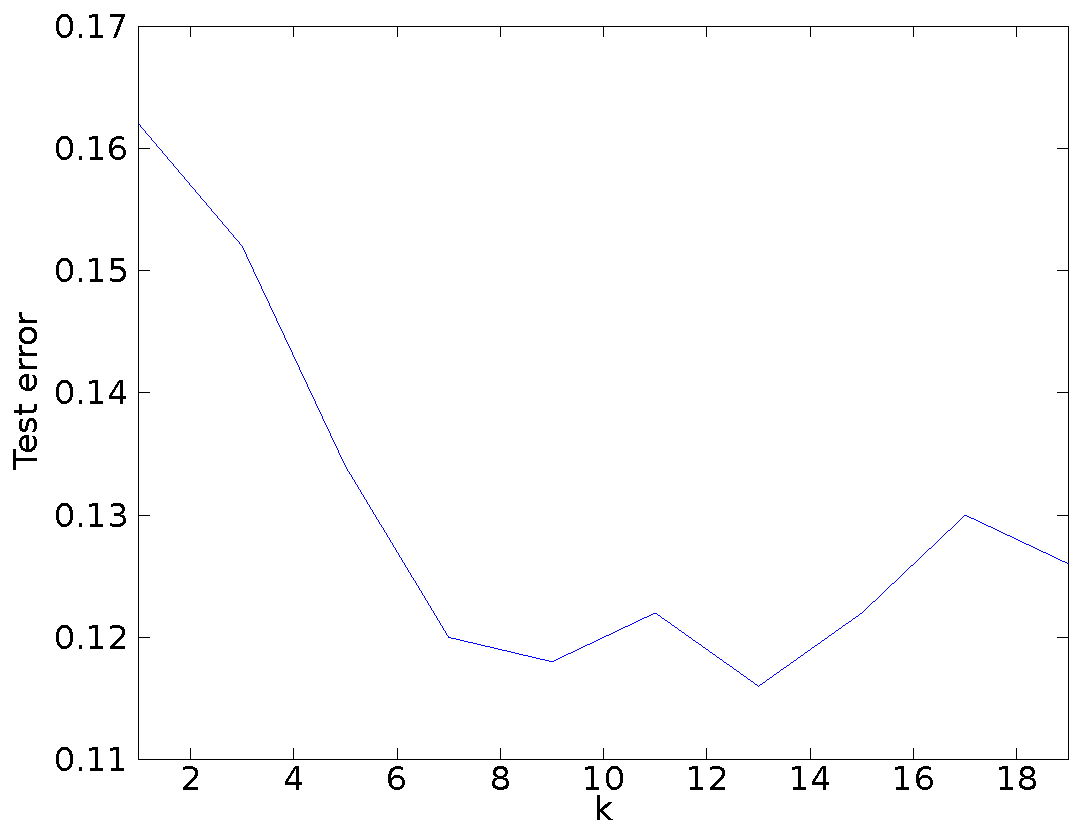
\includegraphics[width=0.6\paperwidth]{plot3.pdf}
  \end{center}
\end{figure}

\Autoref{fig:plot2} shows the test error for $k = 1, 3, \ldots, 999$.  Based on this data, one might choose $\textcolor{\highlightColor}{k = 239}$, as it gives the \textcolor{\highlightColor}{lowest test error}, $0.104$.

However, with a high value for $k$, the classifier is prone to \textcolor{\highlightColor}{overfitting}.  This can be seen in the plot, as the test error goes up for sufficiently high values of $k$.  That we have a low test error for a high value of $k$, might be because of a statistical fluke in the test data.

To avoid overfitting, we might consider a lower value for $k$ with a high accuracy.  For example, $k = 13$ gives an accuracy of $0.116$.  This can be seen in a closeup of the graph in \autoref{fig:plot3}.

Depending on the purpose one might also take the \textcolor{\highlightColor}{recall and precision} into consideration.  

Furthermore, the \textcolor{\highlightColor}{amount of data} is rather \textcolor{\highlightColor}{small} for any real conclusions.

And lastly, the \textcolor{\highlightColor}{test set} is now used \textcolor{\highlightColor}{as a validation set}: we use the test 
error as a manner to chose the parameter $k$ for the model.  
This is troublesome, as a true test error might show a different value for 
$k$; this test set might have a bias towards the value for $k$ we found.
\end{enumerate}

%Confusion matrices of the $k$NN with $1 \leq k \leq 20$:


\section{Cross-validation}
\begin{enumerate}
    \item \textit{Discuss briefly (200 words) what the advantage would be of using a method like cross-validation or
bootstrapping in this context.}

\label{cv}
% Je kunt ook \autoref gebruiken. Zit standaard in hyperref. Ik heb ook een definitie voor \Autoref toegevoegd; dat is \autoref, maar begint dan met een hoofdletter :)
%% OH COOL! :D
\textcolor{\highlightColor}{The available data is very limited}; there are 1000 data points per class.  Plentiful data is preferable over limited 
data.  When one introduces a validation set, the already small data set is 
divided into a training set, test set and a validation set.  This means 
especially, in this situation 
since there already were not that many data points to begin with, 
that the data left to learn from is very little.  \textcolor{\highlightColor}{Smaller validation sets}
are viable but \textcolor{\highlightColor}{give a relatively noisy estimate of predictive performance.}
%TODO: cite pattern recognition and machine learning van christopher m. bishop 

\textcolor{\highlightColor}{Cross-validation is a solution where all the data can be used to train while 
also using all the data to assess performance.}

Cross-validation is a method where one seeks to use the data as efficiently 
as possible.  Another approach when data is limited is 
\textcolor{\highlightColor}{bootstrapping, which 
`creates' more data from the dataset} by randomly selecting data points to 
be duplicated.  And, as always, more data is better, even when it is created
by bootstrapping.  


% The method used in section \ref{sec:two} biases the machine towards the test set.  The test set should normally be
% used to evaluate the machine learning algorithm and/or its parameters.  The test set should not be used to 
% select a model, as was implied in section \ref{sec:two}.  
% Cross-validation can be used to fairly evaluate models using solely the training set without the risk of 
% introducing a bias for one specific validation set.  

\item \textit{Implement 10-fold cross-validation, and give an estimate for a good value of $k$.}

We can run the script ``runme'' once more and use the last two options for 
this part of the assignment.  The following table is the result:

\begin{tabular}{c | c}
\textbf{$k$} & \textbf{Accuracy} \\
\hline
1 &  0.85600\\ 
3 &  0.86600\\ 
5 &  0.87200\\ 
7 &  0.88400\\ 
9 &  0.88000\\ 
11&  0.88200\\ 
13&  0.88200\\ 
15&  0.88600\\ 
17&  0.88400\\ 
19&  0.88600\\ 
21&  0.88200\\ 
23&  0.88600\\ 
25&  0.87800\\ 
\end{tabular}

\textcolor{\highlightColor}{A good value for $k$ seems to be 5} as it as the highest mean accuracy of all
values for $k$.  

\item \textit{Can you use this estimate of $k$ in your final classifier? What is the use of doing cross-validation?}

This is not a good estimation for a good value for $k$, but it is the best 
bet as this value for $k$ shows the best mean accuracy.  The use of doing 
cross-validation is discussed in item \ref{cv} and \ref{cv2} in this section.  

\item \textit{ How do you compute the test error? What is it an estimate of? What would be the use of a validation
set? } 
\label{cv2}
\textcolor{\highlightColor}{The test error is the percentage of data points from the test set which 
are wrongly classified.}

The test set can solely be used to evaluate the (learned) model.  No
information from the test set can be used as feedback in the learning 
process as this would mean that the test set is used to learn from.  
\textcolor{\highlightColor}{The 
test error shows an estimate of how well the model would perform for
any kind of application.}

In section \ref{sec:two} the test set was used to select a $k$.  This is a
typical example of something one should not do: the $k$ could be influenced
by the test set.  

\textcolor{\highlightColor}{ 
The use of a validation set is to investigate different models and/or
parameters without spoiling the test set.}
Different models and parameters can be tested to find those which perform the best on a validation 
set.  Hopefully the results of these tests can be used to select those 
model and parameters which perform best, also on the training set and new 
data in the application for which was learned.  
If the test set was used as the validation set, such 
as in section \ref{sec:two}, the test set could not be used to calculate a 
true error rate because validating models is part of the training process.  

\end{enumerate}

\end{document}



% Run our Matlab script\footnote{This script is also compatible with Octave} 
% ``runme''.  The script asks what you want to run.  The first two options run 
% the code for this exercise.  The first option will use the last part of 
% the data as test data.  The 
% second option will compile a test set by randomly selecting elements from 
% the data until the preferred percentage for the test set has been reached. 
% 
% An example input:
% 
% \begin{verbatim}
% octave:7> runme
% Choose what you want to do
% 
%   [ 1] p% split, with data in order
%   [ 2] p% split, with data shuffled
%   [ 3] n-fold cross-validation, with p% test set and data in order
%   [ 4] n-fold cross-validation, with p% test set and data shuffled
% 
% pick a number, any number: 2
% Which value of k do you want to use? 10
% Which percentage of your data do you want to train on? [0-1> 0.75
% ans =
% 
%    0.84200   0.86400   0.86800   0.88000   0.87600
% \end{verbatim}

% \begin{table}
%   \caption{TA = True A; TB = True B; CA = classified as A; CB = classified as B.}
% \begin{tabular}{lcrr}
% $k$ && CA & CB \\ \\
%  1 & TA & 199 &    51 \\
% & TB &  34 &   216 \\
%  2 & TA & 205 &    45 \\
% & TB &  34 &   216 \\
%  3 & TA & 212 &    38 \\
% & TB &  33 &   217 \\
%  4 & TA & 217 &    33 \\
% & TB &  35 &   215 \\
%  5 & TA & 214 &    36 \\
% & TB &  30 &   220 \\
%  6 & TA & 217 &    33 \\
% & TB &  31 &   219 \\
%  7 & TA & 216 &    34 \\
% & TB &  31 &   219 \\
%  8 & TA & 221 &    29 \\
% & TB &  32 &   218 \\
%  9 & TA & 216 &    34 \\
% & TB &  30 &   220 \\
%  10 & TA & 217 &    33 \\
% & TB &  32 &   218 \\
%  11 & TA & 214 &    36 \\
% & TB &  29 &   221 \\
%  12 & TA & 215 &    35 \\
% & TB &  28 &   222 \\
%  13 & TA & 215 &    35 \\
% & TB &  31 &   219 \\
%  14 & TA & 216 &    34 \\
% & TB &  31 &   219 \\
%  15 & TA & 216 &    34 \\
% & TB &  31 &   219 \\
%  16 & TA & 213 &    37 \\
% & TB &  31 &   219 \\
%  17 & TA & 215 &    35 \\
% & TB &  35 &   215 \\
%  18 & TA & 215 &    35 \\
% & TB &  34 &   216 \\
%  19 & TA & 215 &    35 \\
% & TB &  36 &   214 \\
%  20 & TA & 216 &    34 \\
% & TB &  33 &   217 \\
% \end{tabular}
% \end{table}

